% (c) 2012 Tiziana Manca - tmanca@libero.it
% (c) 2012 -2014 Dimitrios Vrettos - d.vrettos@gmail.com

\section{Esercizi}
\subsection{Esercizi dei singoli paragrafi}
\subsubsection*{\thechapter.1 - Indagine statistica}

\begin{esercizio}
\label{ese:A.1}
In una indagine su alcune famiglie si sono rilevati i seguenti caratteri; indicane il tipo ponendo una crocetta nella casella
opportuna; per i caratteri quantitativi indica se sono discreti o continui, per i caratteri qualitativi indica se sono ordinabili o sconnessi:

\begin{center}
 \begin{tabularx}{.95\textwidth}{p{5.5cm}cccc}
\toprule
Carattere & \multicolumn{2}{c}{quantitativo} & \multicolumn{2}{c}{qualitativo}\\
 & discreto & continuo & ordinabile & sconnesso\\
\midrule
Reddito mensile del capofamiglia & & & & \\
Titolo di studio del capofamiglia & & & & \\
Familiari a carico & & & & \\
Settore lavorativo & & & & \\
Luogo di nascita del capofamiglia & & & & \\
Tempo impiegato per raggiungere il luogo di lavoro & & & & \\
\bottomrule
\end{tabularx}
\end{center}
\end{esercizio}

\subsubsection*{\thechapter.2 - Fasi di un'indagine statistica}

\begin{esercizio}
\label{ese:A.2}
Compila una tabella relativa alla distribuzione degli studenti della tua classe in relazione~a:
\begin{itemize*}
\item colore dei capelli (nero, castano, biondo, rosso);
\item anno di nascita;
\item città di residenza.
\end{itemize*}
\end{esercizio}

\begin{esercizio}
\label{ese:A.3}
In una certa nazione in un dato anno si sono vendute~$\np{10540}$ biciclette, $\np{7560}$ scooter, $\np{2300}$ moto e~$\np{6532}$ automobili. Completa la tabella:
\begin{center}
 \begin{tabularx}{.9\textwidth}{Xccc}
\toprule
Mezzi di trasporto venduti & Freq. assoluta & Freq. relativa & Freq. percentuale \\
\midrule
Biciclette & & & \\
Scooter & & & \\
Moto & & & \\
Automobili & & & \\
\midrule
Totale & & & \\
\bottomrule
\end{tabularx}
\end{center}
\end{esercizio}

\begin{esercizio}
\label{ese:A.4}
Da un'indagine sulla distribuzione delle altezze in un gruppo di studenti sono stati rilevati i seguenti dati grezzi (espressi in~$\unit{cm}$):
\begin{center}
 \begin{tabular}{ccccccccccccc}
175 & 168 & 169 & 173 & 160 & 165 & 170 & 172 & 177 & 172 & 170 & 173 & 182 \\
164 & 174 & 185 & 188 & 164 & 175 & 160 & 177 & 176 & 184 & 180 & 176 & 168 \\
174 & 175 & 177 & 183 & 174 & 166 & 181 & 173 & 166 & 172 & 174 & 165 & 180 \\
190 & 175 & 176 & 188 & 171 & 172 & 181 & 185 & 184 & 183 & 175 & 173 & 181 \\
 \end{tabular}
\end{center}
Raggruppa i dati in classi di ampiezza~$5 \unit{cm}$ e costruisci la distribuzione di frequenza. Calcola poi frequenza relativa e percentuale.
\end{esercizio}

\begin{esercizio}
\label{ese:A.5}
Dall'analisi delle paghe settimanali dei dipendenti di un'industria automobilistica si è ottenuta la seguente distribuzione di frequenza,
suddivisa in classi (la parentesi quadra indica che l'estremo della classe
considerato è incluso nella classe stessa, la parentesi tonda indica che l'estremo della classe considerato è
escluso dalla classe). Determina per ogni classe di reddito frequenza relativa e percentuale.
\begin{center}
 \begin{tabularx}{.9\textwidth}{Xccc}
\toprule
Classi di reddito (\officialeuro) & Freq. assoluta & Freq. relativa & Freq. percentuale \\
\midrule
$[50\text{,~}100)$ & 50 & & \\
$[100\text{,~}200)$ & 70 & & \\
$[200\text{,~}300)$ & 30 & & \\
$\ge~300$ & 50 & & \\
\bottomrule
\end{tabularx}
\end{center}
\end{esercizio}

\begin{esercizio}
\label{ese:A.6}
Data la seguente distribuzione dei risultati dei test d'ingresso di matematica in una scuola media, sapendo che l'indagine è stata svolta su~200 alunni, determina frequenze assolute e relative.
\begin{center}
 \begin{tabularx}{.9\textwidth}{Xccccccc}
\toprule
Voto & 3 & 4 & 5 & 6 & 7 & 8 & 9 \\
Frequenza percentuale & 5\% & 10\% & 25\% & 40\% & 15\% & 3\% & 2\% \\
Frequenza assoluta & & & & & & & \\
Frequenza relativa & & & & & & & \\
\bottomrule
\end{tabularx}
\end{center}
\end{esercizio}

\begin{esercizio}
\label{ese:A.7}
Osserva la seguente tabella:
 \begin{center}
 \begin{tabularx}{.85\textwidth}{lrcc}
\toprule
 & Freq. assoluta & Freq. relativa & Freq. percentuale \\
\midrule
Infanzia & $\np{950000}$ & & \\
Primaria & $\np{2538000}$ & & \\
Secondaria di~1° grado & $\np{1700000}$ & & \\
Secondaria di~2° grado & $\np{2425000}$ & & \\
Totale & & & \\
\bottomrule
\end{tabularx}
 \end{center}
\begin{itemize*}
\item Quale fenomeno descrive la tabella?
\item Qual è la popolazione statistica oggetto dell'indagine?
\item Quante sono le unità statistiche?
\item Qual è stato il carattere indagato?
\item Completa la tabella calcolando frequenza relativa e frequenza percentuale.
\end{itemize*}
\end{esercizio}

\begin{esercizio}
\label{ese:A.8}
In un campione di ginnaste di livello agonistico si è rilevata l'altezza in metri. Questa frase è sufficiente per indicare la popolazione oggetto
di indagine e il carattere rilevato? Il carattere analizzato è di tipo qualitativo o quantitativo?

L'indagine ha dato i seguenti risultati:
\begin{center}
 \begin{tabular}{lccccccccc}
\toprule
Altezza (m) & $\np{1,49}$ & $\np{1,50}$ & $\np{1,55}$ & $\np{1,58}$ & $\np{1,61}$ & $\np{1,64}$ & $\np{1,67}$ & $\np{1,70}$ & $\np{1,71}$ \\
Numero ginnaste & 1 & 6 & 11 & 4 & 6 & 4 & 2 & 2 & 3 \\
\bottomrule
\end{tabular}
\end{center}
Quante sono le unità statistiche? Determina in percentuale il numero delle ginnaste la cui altezza è non inferiore a~$\np[m]{1,60}$.
\end{esercizio}

\begin{esercizio}
\label{ese:A.9}
La tabella mostra dati relativi ad una popolazione di~20 famiglie italiane; le informazioni in essa contenute stabiliscono alcuni aspetti o caratteri
dei membri della popolazione: numero di componenti, reddito annuo (in migliaia di euro), titolo di studio del capofamiglia, residenza per area geografica.
Osserva la tabella e rispondi alle domande che seguono.
\begin{center}
 \begin{tabular}{cccll}
\toprule
Famiglia & Numero componenti & Reddito annuo & Titolo di studio & Residenza\\
\midrule
1 & 2 & 28 & Elementare & Nord \\
2 & 1 & 35 & Media inferiore & Centro \\
3 & 3 & 50 & Media inferiore & Nord \\
4 & 1 & 45 & Media superiore & Nord \\
5 & 1 & 40 & Laurea & Sud \\
6 & 2 & 30 & Media inferiore & Sud \\
7 & 3 & 55 & Media inferiore & Centro \\
8 & 4 & 80 & Media superiore & Centro \\
9 & 5 & 60 & Laurea & Sud \\
10 & 6 & 85 & Laurea & Nord \\
11 & 7 & 90 & Laurea & Nord \\
12 & 1 & 52 & Media superiore & Centro \\
13 & 2 & 62 & Media superiore & Sud \\
14 & 3 & 75 & Media superiore & Sud \\
15 & 5 & 60 & Elementare & Nord\\
16 & 4 & 45 & Media inferiore & Nord \\
17 & 3 & 42 & Media inferiore & Centro \\
18 & 2 & 28 & Elementare & Nord \\
19 & 8 & 70 & Media superiore & Sud \\
20 & 2 & 38 & Laurea & Sud \\
\bottomrule
\end{tabular}
\end{center}
\begin{itemize*}
\item Cosa si intende, in statistica, per popolazione?
\item Quali sono le unità statistiche di cui sono trascritti i dati nella tabella precedente?
\item Quali caratteri riportati nella tabella sono qualitativi e quali quantitativi?
\item Quali sono le modalità dei caratteri qualitativi indagati?
\item Le informazioni della precedente tabella sono sufficienti per stabilire:
\begin{itemize*}
\item dove risiede la maggior parte delle famiglie oggetto di questa indagine? Se sì, come lo stabilisci?
\item il numero di famiglie il cui capofamiglia ha come titolo di studio quello di Scuola Media Superiore? Se sì, come lo stabilisci?
\end{itemize*}
\item costruire la tabella:
\begin{center}
 \begin{tabular}{lllll}
\toprule
Titolo di studio & Elementare & Media inferiore & Media superiore & Laurea \\
Numero di famiglie & & & & \\
\bottomrule
\end{tabular}
\end{center}
\item \`E vero che~$1/4$ dei capifamiglia, cioè il~25\%, è laureato?
\item Costruire un'altra tabella, sul modello della precedente, in cui è riportato il numero di famiglie aventi~1, 2, 3, ecc. componenti.
\`E vero che~$1/3$ delle famiglie è costituito da più di~5 persone?
\item Individua il reddito minimo e quello massimo, completa la seguente tabella delle frequenze in modo che il carattere reddito
sia suddiviso in classi di ampiezza~5, come indicato.
\begin{center}
\begin{tabular}{ll}
\toprule
Classe di reddito & Frequenza assoluta \\
\midrule
26-30 &  \\
31-35 &  \\
\ldots   &  \\
%   &  \\
%   &  \\
\bottomrule
\end{tabular}
\end{center}
\item Quante famiglie hanno un reddito compreso tra~46 e~90 mila euro? Indica la risposta anche in percentuale.
\end{itemize*}
\end{esercizio}

\begin{esercizio}[Fonte Wikipedia]
\label{ese:A.10}
Rappresenta con un diagramma cartesiano la seguente serie storica relativa alla produzione di olio di oliva in Puglia,
scegliendo un'opportuna unità di misura:
\begin{center}
 \begin{tabular}{lcccc}
\toprule
Anno & 2006 & 2005 & 2004 & 2003\\
Produzione olio (quintali) & $\np{1914535}$ & $\np{2458396}$ & $\np{2678201}$ & $\np{2508084}$\\
\bottomrule
\end{tabular}
\end{center}
\end{esercizio}

\begin{esercizio}[Fonte ISTAT]
\label{ese:A.11}
Rappresenta con un diagramma cartesiano la seguente serie storica, relativa al numero di società quotate in borsa, dal~1975 al~1984:
\begin{center}
 \begin{tabular}{lcccccccccc}
\toprule
Anno & 1975 & 1976 & 1977 & 1978 & 1979 & 1980 & 1981 & 1982 & 1983 & 1984 \\
Società & 154 & 156 & 156 & 148 & 145 & 141 & 141 & 148 & 150 & 155 \\
\bottomrule
\end{tabular}
\end{center}
\end{esercizio}

\begin{esercizio}
\label{ese:A.12}
Rappresenta graficamente, mediante diagramma cartesiano, la seguente tabella che riporta le temperature misurate a Lecce durante una giornata invernale.
\begin{center}
\begin{tabularx}{.95\textwidth}{X*{12}{c}}
\toprule
Ore                     & 0 &   2   &   4   & 6 &   8   & 10 & 12 & 14 &   16   & 18 & 20 &  22\\
Temperatura ($\grado$C) & 5 & $\np{5,5}$ & $\np{5,5}$ & 6 & $\np{7,5}$ & 10 & 16 & 18 & $\np{16,5}$ & 12 & 8  & $\np{6,5}$\\
\bottomrule
\end{tabularx}
\end{center}
\end{esercizio}


\begin{esercizio}
\label{ese:A.13}
Rappresenta attraverso un ideogramma la seguente tabella statistica, che indica le ore di studio giornaliere di uno studente,
usando~2 ore come unità di misura. Scegli un simbolo opportuno.
\begin{center}
\begin{tabular}{l*{7}{c}}
\toprule
Giorno & Lunedì & Martedì & Mercoledì & Giovedì & Venerdì & Sabato & Domenica \\
Ore studio & 2 & 6 & 5 & 2 & 3 & 4 & 0 \\
\bottomrule
\end{tabular}
\end{center}
\end{esercizio}

\begin{esercizio}
\label{ese:A.14}
Costruisci un ideogramma a partire dai dati della seguente tabella:
\begin{center}
\begin{tabular}{lc}
\toprule
Regione & Produzione vino (quintali)\\
\midrule
Toscana & $\np{20500}$\\
Veneto & $\np{18000}$\\
Puglia & $\np{15500}$\\
Campania & $\np{14500}$\\
Molise & $\np{8000}$\\
\bottomrule
\end{tabular}
\end{center}
\end{esercizio}

\pagebreak
\begin{esercizio}
\label{ese:A.15}
La seguente tabella rappresenta i risultati di un'indagine sulla capitale europea preferita da un gruppo di studenti universitari.
Rappresenta i dati utilizzando un diagramma a nastro.
\begin{center}
\begin{tabular}{lc}
\toprule
Capitale preferita & Frequenza\\
\midrule
Amsterdam & 28\\
Londra & 30\\
Parigi & 25\\
Roma & 42\\
Vienna & 10\\
\bottomrule
\end{tabular}
\end{center}
\end{esercizio}

\begin{esercizio}
\label{ese:A.16}
Rappresenta con un diagramma a colonne i dati riportati nella seguente tabella relativi alla vendita di automobili da un concessionario nell'anno~2009.
\begin{center}
\begin{tabular}{lc}
\toprule
Marca automobile & Auto vendute\\
\midrule
Alfa Romeo & 30\\
Fiat & 270\\
Ford & 120\\
Renault & 50\\
Toyota & 40\\
\bottomrule
\end{tabular}
\end{center}
\end{esercizio}

\begin{esercizio}
\label{ese:A.17}
Consideriamo la seguente tabella statistica che indica le frequenze percentuali di forza lavoro per settore economico rilevata nel~2006 in Italia:
\begin{center}
\begin{tabular}{lc}
\toprule
Forza lavoro per settore economico & Frequenza percentuale\\
\midrule
Forza lavoro occupata nell'agricoltura & $\np{4,20}\%$\\
Forza lavoro occupata nell'industria & $\np{30,70}\%$\\
Forza lavoro occupata nei servizi & $\np{65,10}\%$\\
Tasso di disoccupazione & $\np{8,00}\%$\\
\bottomrule
\end{tabular}
\end{center}
Rappresentare graficamente mediante areogramma i dati contenuti nella tabella.
\end{esercizio}

\begin{esercizio}
\label{ese:A.18}
Rappresentare attraverso un areogramma la seguente tabella statistica, che indica le altezze di~100 studenti maschi
di una data scuola dopo aver calcolato le frequenze percentuali:
\begin{center}
\begin{tabular}{l*{2}{c}}
\toprule
Altezza (m) & Numero di studenti & Frequenze percentuali\\
\midrule
$\np{1,50}$ - $\np{1,59}$ & 11 & \\
$\np{1,60}$ - $\np{1,69}$ & 18 & \\
$\np{1,70}$ - $\np{1,79}$ & 42 & \\
$\np{1,80}$ - $\np{1,89}$ & 22 & \\
$\np{1,90}$ - $\np{1,99}$ & 6 & \\
\midrule
Totale & 100 & \\
\bottomrule
\end{tabular}
\end{center}

\end{esercizio}

\begin{esercizio}
\label{ese:A.19}
Rappresentare attraverso un istogramma la seguente tabella statistica, che indica le altezze di~100 studenti maschi di una data scuola:
\begin{center}
\begin{tabular}{l*{5}{c}}
\toprule
Altezza (m) & $\np{1,50}$ - $\np{1,59}$ & $\np{1,60}$ - $\np{1,69}$ & $\np{1,70}$ - $\np{1,79}$ & $\np{1,80}$ - $\np{1,89}$ & $\np{1,90}$ - $\np{1,99}$\\
Numero di studenti & 11 & 18 & 42 & 22 & 6 \\
\bottomrule
\end{tabular}
\end{center}
\end{esercizio}

\begin{esercizio}
\label{ese:A.20}
Uno studente universitario di Matematica ha superato~28 esami con queste valutazioni:
\begin{center}
 \begin{tabular}{cccccccccccccc}
18 & 25 & 26 & 23 & 30 & 21 & 24 & 20 & 29 & 28 & 24 & 21 & 23 & 28\\
28 & 24 & 22 & 25 & 24 & 27 & 24 & 21 & 23 & 28 & 18 & 25 & 26 & 23\\
 \end{tabular}
\end{center}
Organizza i dati in una tabella suddividendoli in classi e rappresentali tramite un istogramma.
\end{esercizio}

\subsubsection*{\thechapter.3 - Indici di posizione}

\begin{esercizio}
\label{ese:A.21}
Un concessionario vende delle moto di diversa cilindrata come descritto nella tabella.
Determinare la moda.
\begin{center}
\begin{tabular}{l*{5}{c}}
\toprule
Cilindrata & 250 &350 &500 &750 &1000\\
Numero moto vendute & 34 & 30 & 45 & 100 & 42 \\
\bottomrule
\end{tabular}
\end{center}
\end{esercizio}

\begin{esercizio}
\label{ese:A.22}
Calcolare la moda della distribuzione rappresentata attraverso la seguente tabella statistica:
\begin{center}
 \begin{tabular}{l*{6}{c}}
\toprule
Modalità del carattere & 3 & 6 & 8 & 9 & 12 & 24 \\
Frequenza & 23 & 78 & 67 & 78 & 89 & 100 \\
\bottomrule
\end{tabular}
\end{center}
\end{esercizio}

\begin{esercizio}
\label{ese:A.23}
Calcolare la classe modale della seguente distribuzione:
\begin{center}
\begin{tabular}{l*{5}{c}}
\toprule
Abitanti & 0 - $999$& $\np{1000}$ - $\np{1999}$& $\np{2000}$ - $\np{4999}$ & $\np{5000}$ - $\np{9999}$& $\np{10000}$ - $\np{19999}$ \\
Numero comuni & $750$ & $\np{1100}$ & $950$ & $\np{2500}$ & $\np{3000}$ \\
\bottomrule
\end{tabular}
\end{center}
\end{esercizio}

\begin{esercizio}[\Ast]
\label{ese:A.24}
Trovare la media aritmetica semplice delle seguenti serie di osservazioni:
\begin{multicols}{2}
\begin{enumeratea}
 \item 3, 4, 6, 7, 10;
 \item 6, 7, 8, 12, 15, 22;
 \item 34, 53, 45, 67, 87, 90, 100, 123.
\end{enumeratea}
\end{multicols}
\end{esercizio}

\begin{esercizio}
\label{ese:A.25}
In una classe di~15 ragazzi sono stati rilevati i seguenti pesi in~$\unit{kg}$:
50, 43, 62, 41, 70, 55, 76, 43, 46, 50, 78, 62, 49, 55, 48.
Calcola la media aritmetica semplice del peso dei ragazzi. Costruisci la tabella delle frequenze.
Calcola la media aritmetica ponderata del peso dei ragazzi. Che cosa osservi?
\end{esercizio}

\begin{esercizio}[\Ast]
\label{ese:A.26}
In un insieme di numeri compaiono quattro volte il~3, cinque volte il~5, tre volte il~6, due volte il~10, due volte il~15. Calcolare la media aritmetica.
\end{esercizio}

\begin{esercizio}[\Ast]
\label{ese:A.27}
Calcola la media della seguente distribuzione di frequenza.
\begin{center}
 \begin{tabular}{l*{6}{c}}
\toprule
Punteggio & 2 & 4 & 6 & 7 & 12 & 14 \\
Frequenza assoluta & 2 & 4 & 5 & 4 & 3 & 2 \\
\bottomrule
\end{tabular}
\end{center}
\end{esercizio}

\begin{esercizio}
\label{ese:A.28}
Una rivista di auto fornisce i seguenti punteggi per tre diversi modelli di automobili.
\begin{center}
 \begin{tabular}{l*{5}{c}}
\toprule
 & Funzionalità & Volumetria & Prestazioni & Sicurezza & Economia \\
\midrule
Modello~1 & $\np{2,5}$ & $4$ & $\np{3,2}$ & $\np{3,5}$ & $\np{2,5}$ \\
Modello~2 & $\np{2,5}$ & $3$ & $4$ & $\np{3,5}$ & $2$ \\
Modello~3 & $\np{2,7}$ & $3$ & $\np{3,5}$ & $\np{3,8}$ & $\np{2,5}$ \\
\bottomrule
\end{tabular}
\end{center}
Quale tipo di auto viene considerato mediamente migliore se si dà lo stesso peso alle singole caratteristiche?
\end{esercizio}

\begin{esercizio}
\label{ese:A.29}
Un insegnante di fisica, per mostrare che le misure di uno stesso oggetto sono soggette ad errori che dipendono dall'osservatore,
ha fatto misurare la lunghezza di una cattedra con un metro a ciascun alunno della propria classe. I risultati sono stati i seguenti:
\begin{center}
 \begin{tabular}{l*{5}{c}}
\toprule
Lunghezza (cm) & $\np{100,8}$ & $\np{100,9}$ & $\np{101,2}$ & $\np{101,5}$ & $\np{102}$\\
Frequenza & 2 & 8 & 5 & 4 & 1\\
\bottomrule
\end{tabular}
\end{center}
Qual è la lunghezza media della cattedra?
\end{esercizio}

\begin{esercizio}[\Ast]
\label{ese:A.30}
Trovare la mediana delle seguenti serie di osservazioni:
\begin{multicols}{2}
\begin{enumeratea}
 \item 3, 4, 6, 7, 10;
 \item 6, 7, 8, 12, 15, 22;
 \item 34, 53, 45, 67, 87, 91, 100, 123, 129, 135.
\end{enumeratea}
\end{multicols}
\end{esercizio}

\begin{esercizio}[\Ast]
\label{ese:A.31}
In una classe di~15 ragazzi sono stati rilevati i seguenti pesi in~$\unit{kg}$:
50, 43, 62, 41, 70, 55, 76, 43, 46, 50, 78, 62, 49, 55, 48.
Calcola la mediana del peso dei ragazzi.
\end{esercizio}

\begin{esercizio}[\Ast]
\label{ese:A.32}
Dati i seguenti tempi di risposta ad un test sostenuto da un gruppo di~8 studenti ad un concorso
in un ente pubblico~19, 25, 20, 15, 8, 5, 12, 15, calcola la mediana.
\end{esercizio}

\begin{esercizio}
\label{ese:A.33}
Calcola la classe mediana sulla base dei dati riportati nella tabella seguente relativa agli occupati nel settore agricolo suddivisi per età:
\begin{center}
 \begin{tabular}{l*{5}{c}}
\toprule
Età & 20-25 & 25-30 & 30-35 & 35-40 & Oltre~40\\
Frequenza & 500 & 750 & 230 & 400 & 350\\
\bottomrule
\end{tabular}
\end{center}
\end{esercizio}

\subsubsection*{\thechapter.4 - Indici di variabilità}

\begin{esercizio}
\label{ese:A.34}
Calcola campo di variazione e varianza della seguente distribuzione:~$6$, $8$, $10$, $12$, $14$.
\end{esercizio}

\begin{esercizio}
\label{ese:A.35}
Nella seguente tabella sono indicati i consumi bimestrali d'acqua, espressi in metri cubi, di una certa famiglia in due anni consecutivi:
\begin{center}
 \begin{tabular}{l*{6}{c}}
\toprule
Bimestre & 1 & 2 & 3 & 4 & 5 & 6 \\
\midrule
Consumo anno~1 ($\unit{m}^3$) & 70 & 80 & 110 & 120 & 140 & 90 \\
Consumo anno~2 ($\unit{m}^3$) & 80 & 75 & 100 & 130 & 120 & 85 \\
\bottomrule
\end{tabular}
\end{center}
Calcola, per ciascun anno, media, campo di variazione e varianza. Stabilisci infine, giustificando la risposta, in quale anno c'è stata una variabilità maggiore.
\end{esercizio}

\begin{esercizio}
\label{ese:A.36}
In un gruppo di studenti la valutazione dell'esame di biologia risulta così distribuita:
$27$, $25$, $26$, $24$, $24$, $21$, $24$, $20$, $29$, $28$,
$28$, $24$, $22$, $25$, $24$, $22$, $24$, $21$, $23$, $28$.
\begin{enumeratea}
 \item Organizza i dati in una tabella, indicando anche la frequenza assoluta, quella relativa in frazione e quella percentuale;
 \item rappresenta i dati in un grafico a piacere;
 \item calcola moda, media e mediana dandone una breve interpretazione;
 \item calcola la varianza.
\end{enumeratea}
\end{esercizio}

\begin{esercizio}
\label{ese:A.37}
Una ditta paga~5 persone \officialeuro~$165$ alla settimana, 4 persone\officialeuro~$199$ alla settimana e~2 persone \officialeuro~$218$ alla settimana.
Trova media aritmetica, moda e mediana. Che percentuale di persone ha la retribuzione che si discosta,
sia in positivo che in negativo, di \officialeuro~$20$ dalla media?
\end{esercizio}

\begin{esercizio}
\label{ese:A.38}
\`E stata effettuata un'indagine statistica fra le persone presenti in una libreria riguardo al numero di libri letti
nella scorsa estate. I dati sono raccolti nella seguente tabella:
\begin{center}
 \begin{tabular}{l*{8}{c}}
\toprule
N° libri letti & 0 & 1 & 2 & 3 & 4 & 5 & 6 & 7 \\
N° persone & 20 & 35 & 9 & 6 & 3 & 0 & 1 & 1 \\
\bottomrule
\end{tabular}
\end{center}
\begin{enumeratea}
 \item Organizza i dati in una tabella e calcola la frequenza assoluta, quella relativa e quella percentuale;
 \item rappresenta i dati in un grafico scelto a piacere;
 \item calcola moda, media e mediana dandone una semplice interpretazione;
 \item calcola varianza e coefficiente di variazione.
\end{enumeratea}
\end{esercizio}

\subsection{Esercizi riepilogativi}
\begin{esercizio}
\label{ese:A.39}
Scegli la risposta corretta:
\begin{enumerate*}
 \item se compi un'indagine sul peso degli allievi della tua scuola, la popolazione è costituita
 \begin{enumeratea}
 \item dagli allievi della scuola;
\item dai pesi degli allievi della tua scuola;
\item da ciascun allievo della scuola;
\item dal peso di ciascun allievo della scuola.
 \end{enumeratea}
 \item nella stessa indagine, da cosa sarà costituita un'unità statistica?
 \begin{enumeratea}
 \item dagli allievi della scuola;
\item dai pesi degli allievi della tua scuola;
\item da ciascun allievo della scuola;
\item dal peso di ciascun allievo della scuola.
 \end{enumeratea}
\item un'indagine statistica realizzata intervistando solo una parte della popolazione statistica è definita
 \begin{enumeratea}
 \item incompleta;
\item universo;
\item censimento;
\item a campione;
 \end{enumeratea}
\item la frequenza percentuale si ottiene
 \begin{enumeratea}
\item dividendo la frequenza per il totale delle frequenze e moltiplicando il risultato per~100;
\item moltiplicando la frequenza per~100;
\item moltiplicando la frequenza per il totale delle frequenze e dividendo il risultato per~100;
\item dividendo la frequenza per~100.
 \end{enumeratea}
\item la mediana:
 \begin{enumeratea}
\item è il valore che si ottiene dividendo la somma dei valori delle singole osservazioni per il loro numero;
\item è il valore equidistante dagli estremi di un insieme di dati ordinati;
\item è il valore che si presenta con la massima frequenza in un insieme di dati;
\item è il valore che indica la percentuale di dati al di sopra o al di sotto della media.
 \end{enumeratea}
\item la media aritmetica:
 \begin{enumeratea}
 \item è il valore che si ottiene dividendo la somma dei valori delle singole osservazioni per il loro numero;
\item è il valore equidistante dagli estremi di un insieme di dati ordinati;
\item è il valore che si presenta con la massima frequenza in un insieme di dati;
\item è il valore che indica la percentuale di dati al di sopra o al di sotto della media.
 \end{enumeratea}
\item la moda:
 \begin{enumeratea}
\item è il valore che si ottiene dividendo la somma dei valori delle singole osservazioni per il loro numero;
\item è il valore equidistante dagli estremi di un insieme di dati ordinati;
\item è il valore che si presenta con la massima frequenza in un insieme di dati;
\item è il valore che indica la percentuale di dati al di sopra o al di sotto della media.
 \end{enumeratea}
\item nella seguente distribuzione di dati~2, 4, 4, 4, 4, 6, 6, 6, 7, 7, quale delle seguenti affermazioni è corretta?
 \begin{enumeratea}
\item la media aritmetica è~5, la moda è~4, la mediana è~6;
\item la media aritmetica è~4, la moda è~6, la mediana è~5;
\item la media aritmetica è~5, la moda è~6, la mediana è~4;
\item la media aritmetica è~5, la moda è~4, la mediana è~5.
 \end{enumeratea}
\item nella tua classe la mediana dell'altezza è~$152\unit{cm}$. Questo significa che:
 \begin{enumeratea}
\item non ci sono studenti più bassi di~$152\unit{cm}$;
\item $152\unit{cm}$ è l'altezza più comune;
\item la metà degli studenti ha un'altezza inferiore a~$152\unit{cm}$, mentre l'altra metà ha un'altezza superiore;
\item in media gli studenti sono alti~$152\unit{cm}$.
 \end{enumeratea}
\item nella tua classe la moda dell'altezza è~$152\unit{cm}$. Questo significa che:
 \begin{enumeratea}
\item non ci sono studenti più bassi di~$152\unit{cm}$;
\item $152\unit{cm}$ è l'altezza più comune;
\item la metà degli studenti ha un'altezza inferiore a~$152\unit{cm}$, mentre l'altra metà l'ha superiore;
\item in media gli studenti sono alti~$152\unit{cm}$.
 \end{enumeratea}
\item nella tua classe la media aritmetica dell'altezza è~$152\unit{cm}$. Questo significa che:
 \begin{enumeratea}
\item non ci sono studenti più bassi di~$152\unit{cm}$;
\item $152\unit{cm}$ è l'altezza più comune;
\item la metà degli studenti ha un'altezza inferiore a~$152\unit{cm}$, mentre l'altra metà l'ha superiore;
\item se tutti gli alunni avessero la stessa altezza questa sarebbe di~$152\unit{cm}$.
 \end{enumeratea}

\end{enumerate*}
\end{esercizio}
\pagebreak
\begin{esercizio}
\label{ese:A.40}
In un test sulla prova di velocità di lettura i candidati hanno ottenuto i seguenti risultati:
\begin{center}
 \begin{tabularx}{.7\textwidth}{X*{7}{c}}
\toprule
N° pagine lette in~15 minuti & 10 & 12 & 11 & 9 & 14 & 13 & 7 \\
N° candidati & 2 & 5 & 2 & 1 & 1 & 3 & 4 \\
\bottomrule
\end{tabularx}
\end{center}
\begin{enumeratea}
 \item Organizza i dati in una tabella indicando frequenza assoluta, frequenza relativa e percentuale;
 \item rappresenta i dati in un diagramma a bastoni;
 \item calcola moda, media e mediana;
 \item quanti candidati in percentuale hanno letto un numero di pagine sopra la media?
\end{enumeratea}
\end{esercizio}

\begin{esercizio}
\label{ese:A.41}
In un gruppo di ragazzi le stature (espresse in centimetri) risultano distribuite nel seguente modo:
163, 169, 171, 165, 173, 165, 163, 168,
168, 169, 171, 169, 181, 165, 168, 169,
169, 163, 169, 168, 150, 168, 172, 181,
165, 169, 172, 169, 192, 173, 163, 168.

\begin{enumeratea}
 \item Costruisci una tabella indicando i dati, la loro frequenza, la frequenza relativa e la percentuale;
 \item suddividi i dati in~4 classi, costruisci la distribuzione di frequenza e rappresentali graficamente con un istogramma;
 \item calcola la moda, la media e la mediana.
\end{enumeratea}
\end{esercizio}

\begin{esercizio}
\label{ese:A.42}
Sono state misurate le pulsazioni al minuto di~20 persone ottenendo i seguenti dati:
79, 72, 69, 69, 72, 80, 73, 73, 70, 66,
80, 68, 70, 72, 82, 75, 72, 71, 74, 64.

\begin{enumeratea}
 \item Organizza i dati in una tabella comprensiva di percentuale di frequenze;
 \item rappresenta graficamente i dati;
 \item calcola moda, media e mediana.
\end{enumeratea}
\end{esercizio}

\begin{esercizio}
\label{ese:A.43}
Ventuno ragazzi sono stati sottoposti a una verifica; i dati seguenti esprimono il numero di errori commessi da ciascuno
di loro: 3, 4, 1, 3, 6, 6, 3, 1, 4, 7, 3, 1, 1, 3, 7, 7, 1, 3, 7, 3, 3.
\begin{enumeratea}
 \item Organizza i dati in una tabella comprensiva di percentuale di frequenze;
 \item rappresenta graficamente i dati;
 \item calcola moda, media e mediana;
 \item quanti alunni, in percentuale, hanno fatto meno di~5 errori?
\end{enumeratea}
\end{esercizio}

\begin{esercizio}
\label{ese:A.44}
I dati riportati in tabella si riferiscono ai giorni di assenza degli alunni di una classe.
\begin{center}
 \begin{tabular}{*{4}{lc}}
\toprule
Alunno & n° giorni & Alunno & n° giorni & Alunno & n° giorni & Alunno & n° giorni\\
\midrule
Mauro & 5 & Romeo & 2 & Bruna & 7 & Silvia & 2\\
Antonio & 7 & Anna & 4 & Pietro & 2 & Alessio & 2\\
Paola & 5 & Luca & 4 & Nicola & 7 & Patrizia & 9\\
Luisa & 5 & Amedeo & 5 & Aldo & 2 & Franca & 1\\
Carla & 1 & Marco & 7 & Luigi & 2 & Chiara & 7\\
\bottomrule
\end{tabular}
\end{center}
\begin{enumeratea}
 \item Organizza i dati in una tabella comprensiva di percentuale di frequenze;
 \item rappresenta i dati con un istogramma;
 \item calcola moda, media e mediana;
 \item quanti alunni, in percentuale, hanno fatto meno assenze rispetto alla media?
\end{enumeratea}
\end{esercizio}

\begin{esercizio}
\label{ese:A.45}
Nella tabella sono riportati i punteggi ottenuti da~22 alunni in un test formato da~20 quesiti a scelta multipla e il numero di risposte esatte.
\begin{center}
\begin{tabular}{*{2}{lcc}}
\toprule
N° ordine & Punteggi & Risposte esatte &N° ordine & Punteggi & Risposte esatte\\
\midrule
1 & 80 & 26 &12 & 55 & 11 \\
2 & 62 & 12 &13 & 58 & 11 \\
3 & 48 & 9 &14 & 80 & 16 \\
4 & 71 & 14 &15 & 75 & 14 \\
5 & 80 & 16 &16 & 65 & 12 \\
6 & 90 & 18 &17 & 58 & 11 \\
7 & 75 & 15 &18 & 58 & 10 \\
8 & 67 & 13 &19 & 62 & 12 \\
9 & 79 & 15 &20 & 57 & 11 \\
10 & 62 & 12 &21 & 60 & 12 \\
11 & 95 & 19 &22 & 48 & 8 \\
\bottomrule
\end{tabular}
\end{center}
\begin{enumeratea}
 \item Il punteggio medio è stato~$\dots$ con uno scarto quadratico medio di~$\dots$;
 \item la mediana della distribuzione è il punteggio~$\dots$;
 \item le risposte esatte sono state in media~$\dots$ con uno scarto quadratico di~$\dots$;
 \item rappresenta ciascuna distribuzione con un istogramma, dopo aver aggregato i dati in classi come indicato nelle tabelle sottostanti.
\end{enumeratea}

\begin{center}
\begin{tabular}{*{2}{lc}}
\toprule
\multicolumn{2}{c}{Carattere~$\dots$} & \multicolumn{2}{c}{Carattere~$\dots$} \\
Punteggio & Frequenza assoluta & Risposte esatte & Frequenza assoluta \\
\midrule
$48 \leq \text{p} < 58$ &  & $7 \leq \text{r.e.} < 9$ & \\
$58 \leq \text{p} < 68$ &  & $9 \leq \text{r.e.} < 11$ & \\
$68 \leq \text{p} < 78$ &  & $11 \leq \text{r.e.} < 13$ & \\
$78 \leq \text{p} < 88$ &  & $13 \leq \text{r.e.} < 15$ & \\
$88 \leq \text{p} < 98$ &  & $15 \leq \text{r.e.} < 17$ & \\
 &  & $17 \leq \text{r.e.} < 19$ & \\
 &  & $19 \leq \text{r.e.} < 21$ & \\
 \midrule
Totale & & Totale & \\
\bottomrule
\end{tabular}
\end{center}
\end{esercizio}

\begin{esercizio}
\label{ese:A.46}
Una scatola contiene~20 sacchetti di biscotti confezionati da una industria. I pesi rilevati in~$\unit{grammi}$ sono:
380, 365, 371, 375, 376, 369, 376, 377, 381, 383, 384, 377, 370, 375, 374, 376, 373, 378, 383, 378.
\begin{enumeratea}
 \item Il carattere rilevato è~$\ldots$, esso è di tipo~$\ldots$ e si presenta secondo modalità~$\ldots$.
 Inserisci nella tabella sottostante nella colonna~$C1$ il carattere rilevato e le sue modalità;
 \item quanto è il peso totale della scatola? Come lo hai calcolato?
 \item il peso medio dei sacchetti di biscotti è~$\media = \ldots$;
 \item qual è il campo di variazione del peso dei sacchetti? $\cvar = \ldots$;
 \item la mediana della distribuzione è~$\ldots$;
 \item nella colonna ``scarto'' riporta, per ciascun valore del carattere indagato, lo scarto dalla media.
 Verifica la proprietà degli scarti rispetto rispetto alla media: la loro somma è~$\ldots$;
 \item completa la colonna~$\vert$scarto$\vert$ con il valore assoluto degli scarti e determina lo scarto medio assoluto~$s = \dots$;
 \item completa la colonna scarto$^2$ con il quadrato degli scarti e calcola la varianza~$\var = \ldots$ e
 il coefficiente di variazione~$\cfvar = \ldots$;
 \item raggruppa i valori del carattere in classi di ampiezza~$5 \unit{gr}$ e completa la tabella;
 \item metti in evidenza la classe modale e spiega il significato di moda;
 \item costruisci l'istogramma della distribuzione;

\begin{center}
\begin{tabular}{*{2}{lcccc}}
\toprule
 & $C1$ & scarto &$\vert$scarto$\vert$ &scarto$^2$& & $C1$ & scarto &$\vert$scarto$\vert$ &scarto$^2$\\
\midrule
1 & & & & &11 & & & &\\
2 & & & & &12 & & & &\\
3 & & & & &13 & & & &\\
4 & & & & &14 & & & &\\
5 & & & & &15 & & & &\\
6 & & & & &16 & & & &\\
7 & & & & &17 & & & &\\
8 & & & & &18 & & & &\\
9 & & & & &19 & & & &\\
10 & & & & &20 & & & &\\
\midrule
Totale & & & &&&&\\
\bottomrule
\end{tabular}
\end{center}

\item organizza i dati in classi:
\begin{center}
\begin{tabular}{lc}
\toprule
Classi di peso & Frequenza assoluta\\
\midrule
$[365$, $370)$ & \\
\ldots & \\
\bottomrule
\end{tabular}
\end{center}
\end{enumeratea}
\end{esercizio}

\begin{esercizio}
\label{ese:A.47}
Dai dati di scrutinio del primo quadrimestre in una scuola secondaria di~2° grado, è stata elaborata la seguente tabella in cui compaiono i voti in matematica degli alunni delle classi prime:
\begin{center}
\begin{tabular}{l*{9}{c}}
\toprule
Voto&3 &4 &5 &6 &7 &8 &9 &10 &Totale\\
Frequenza &1&3&5&7&2&3&1&1&\\
Frequenza relativa&&&&&&&&&\\
Frequenza percentuale&&&&&&&&&\\
\bottomrule
\end{tabular}
\end{center}
\begin{enumeratea}
 \item Indica il numero di unità statistiche oggetto dell'indagine e spiega come lo puoi ottenere;
 \item il carattere rilevato è~$\dots$; esso è di tipo~$\dots$ e si presenta secondo modalità~$\dots$;
 \item la tabella assegnata è di dati aggregati o disaggregati?
 \item rappresenta la distribuzione attraverso un grafico a barre (o a nastro);
 \item cosa si intende per frequenza assoluta?
 \item completa la colonna della frequenza relativa;
 \item completa la colonna frequenza percentuale;
 \item determina la moda della distribuzione:~$\moda = \dots$;
 \item il voto medio in matematica alla fine del primo quadrimestre è stato~$\dots$;
 \item determina la mediana della distribuzione:~$\mediana= \dots$;
 \item amplia la tabella indicando gli scarti dalla media;
 \item calcola lo scarto medio assoluto e lo scarto quadratico medio;
 \item il voto medio dei ragazzi sufficienti è stato~$\dots$, quello dei ragazzi insufficienti è stato~$\dots$;
 \item rappresenta la situazione con un areogramma distinguendo tra ragazzi sufficienti e ragazzi insufficienti.
 \end{enumeratea}
\end{esercizio}

\begin{esercizio}[Prove Invalsi~2011]
\label{ese:A.48}
Il reddito medio annuo dei lavoratori agricoli di un certo paese ammonta a~$3\,500$ scudi e quello dei lavoratori dell'industria
a~$4\,500$ scudi. È corretto affermare che il reddito medio complessivo ammonta a~$4\,000$ scudi?
\end{esercizio}

\begin{esercizio}[\Ast Prove Invalsi~2011]
\label{ese:A.49}
La settimana scorsa la mamma chiese ad Aurelia di trascrivere al computer un manoscritto e Aurelia le assicurò che avrebbe
battuto~20 pagine al giorno. Per la prima metà del manoscritto andò piuttosto lentamente battendo~10 pagine al giorno e poi,
per recuperare il tempo perduto, trascrisse la seconda metà a~30 pagine al giorno.
Quando ebbe finito portò a sua madre la trascrizione dicendole: Vedi, ho fatto una media di~20 pagine al giorno,
come ti avevo promesso. Infatti~$(10+30)/2=20$. Non è vero, replicò sua madre.
\end{esercizio}

\begin{esercizio}[\Ast Prove Invalsi~2011]
\label{ese:A.50}
In una indagine sullo stato di salute della popolazione sono state raccolte informazioni relative al peso e
alla statura di~$1\,000$ intervistati. Gli intervistati sono stati poi suddivisi in quattro gruppi,
come riportato nel grafico seguente. Quante sono le persone in sovrappeso?

\begin{enumeratea}
 \item Più di~500, ma meno di~600;
 \item più di~600;
 \item meno della somma delle persone sottopeso e obese;
 \item all'incirca tante quante sono le persone normopeso.
\end{enumeratea}
\begin{center}
 % (c) 2012 Dimitrios Vrettos - d.vrettos@gmail.com

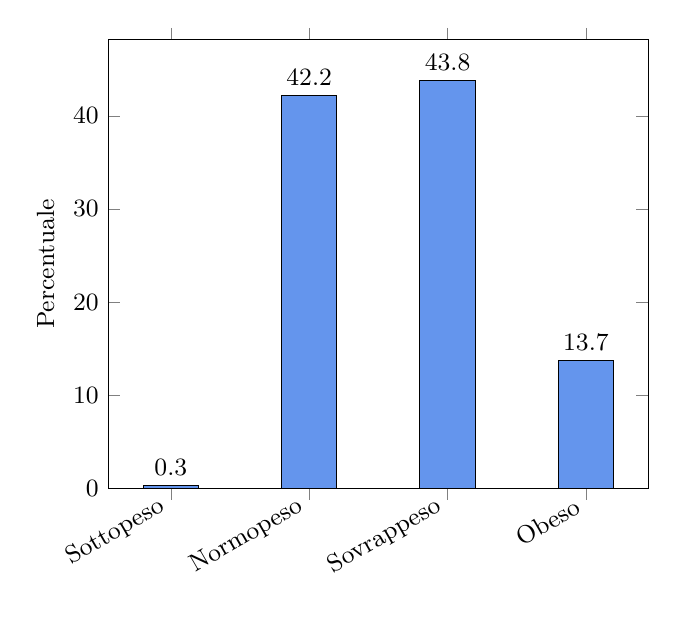
\begin{tikzpicture}[font=\small]
\begin{axis}[ymin=0,
ybar,
xtick=data,
ylabel=Percentuale,
x tick label style={rotate=30,anchor=east},
symbolic x coords={Sottopeso, Normopeso, Sovrappeso, Obeso},
bar width=20pt,enlarge x limits=0.15,nodes near coords,
nodes near coords align={vertical},
]
    \addplot[fill=CornflowerBlue,draw=black]
      coordinates{
	(Sottopeso, .3)
(Normopeso, 42.2)
(Sovrappeso, 43.8)
(Obeso,13.7)
      };
\end{axis}
\end{tikzpicture}

\end{center}

\end{esercizio}

\begin{esercizio}
\label{ese:A.51}
Quattro amici sostengono l'Esame di Stato conseguendo punteggi la cui media aritmetica è~$\np{77,5}/100$.
Se tre di essi hanno conseguito un punteggio, in centesimi, rispettivamente di~70, 76, 80, quale punteggio ha conseguito il quarto studente?
\end{esercizio}
\pagebreak
\begin{esercizio}[Prove Invalsi~2004-2005]
\label{ese:A.52}
La seguente tabella si riferisce alla rilevazione effettuata in una classe prima di un Istituto Tecnico.
\begin{center}
 \begin{tabular}{l*{4}{c}}
\toprule
 & \multicolumn{4}{c}{Scuola media di provenienza}\\
Sesso & Scuola A & Scuola B & Scuola C & Altre scuole\\
\midrule
Maschi & 5 & 3 & 4 & 2 \\
Femmine & 6 & 3 & 4 & 3 \\
\bottomrule
\end{tabular}
\end{center}
Qual è la percentuale di alunni provenienti dalla Scuola B?
\end{esercizio}

\begin{esercizio}[Prove Invalsi~2005-2006]
\label{ese:A.53}
In una classe di~25 alunni, i punteggi (abbreviati in tabella con~$p$) ottenuti in un test di matematica risultano distribuiti come indicato nella seguente tabella.
\begin{center}
 \begin{tabular}{l*{5}{c}}
\toprule
Punteggio & $0 \leq p < 20$ & $20 \leq p < 40$ & $40 \leq p < 60$ & $60 \leq p < 80$ & $80 \leq p \leq~100$ \\
Numero alunni & & & & & \\
\bottomrule
\end{tabular}
\end{center}
Qual è la percentuale di alunni che ha ottenuto un punteggio inferiore a~60?
\end{esercizio}

\begin{esercizio}[Prove Invalsi~2005-2006]
\label{ese:A.54}
Un impiegato ha percepito per i primi~3 mesi dell'anno uno stipendio mensile di \officialeuro~$850$. Nei~9 mesi successivi ha percepito
lo stipendio mensile precedente aumentato di\officialeuro~$200$. Quant'è lo stipendio medio nell'anno di quell'impiegato?
\end{esercizio}

\begin{esercizio}[Prove Invalsi~2005-2006]
\label{ese:A.55}
Nel grafico seguente si riporta l'età dei ragazzi che frequentano una palestra. Qual è la media aritmetica dell'età dei ragazzi
se la distribuzione di frequenza è quella indicata nel grafico?
\begin{center}
 % (c) 2012 Dimitrios Vrettos - d.vrettos@gmail.com
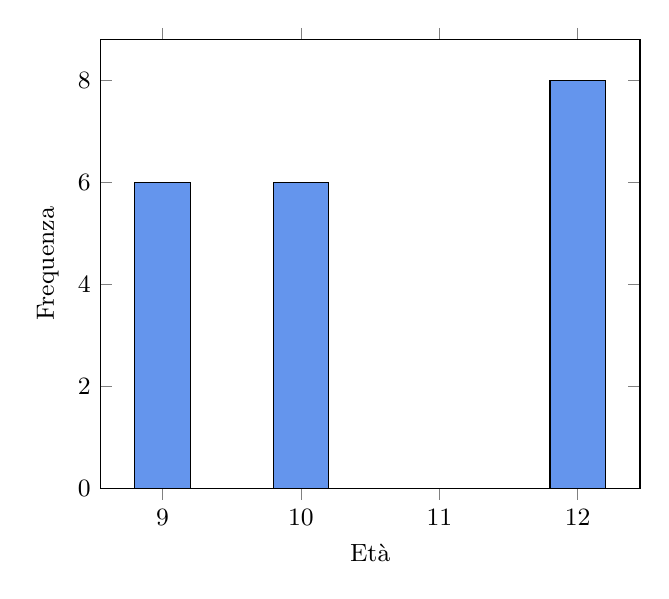
\begin{tikzpicture}[font=\small]

\begin{axis}[ymin=0,
ybar,
ylabel=Frequenza,
xlabel=Età,
bar width=20pt,
enlarge x limits=0.15,]

\addplot[fill=CornflowerBlue,draw=black]
      coordinates{
	(9, 6)
	(10,6)
	(12,8) };
\end{axis}
\end{tikzpicture}

\end{center}
\end{esercizio}
\pagebreak
\begin{esercizio}[Prove Invalsi~2006-2007]
\label{ese:A.56}
I~25 alunni della terza~$C$, dopo aver raccolto i voti conseguiti
nella verifica scritta di matematica, hanno costruito il seguente grafico:
\begin{center}
 % (c) 2012 Dimitrios Vrettos - d.vrettos@gmail.com


\begin{tikzpicture}[x=10mm,y=10mm, x radius=10mm, y radius=10mm]
  \draw (0,0) circle (3);
  \draw[fill=orange] (0,0) -- (0:3) arc (0:14.4:3);
 \draw[fill=brown] (0,0)-- (14.4:3) arc (14.4:57.6:3);
 \draw[fill=green] (0,0)-- (57.6:3) arc (57.6:158.4:3);
\draw[fill=red] (0,0)-- (158.4:3) arc (158.4:273.6:3);
 \draw[fill=blue] (0,0)-- (273.6:3) arc (273.6:316.8:3);
 \draw[fill=olive] (0,0)-- (316.8:3) arc (316.8:345.6:3);
 \draw[fill=lightgray] (0,0)-- (345.6:3) arc (345.6:360:3);

\node[above]  at (0,3) {Voti di Matematica della classe terza $C$};
\begin{scope}[xshift=50mm,
every node/.style={ anchor=center}]
\matrix[matrix of nodes] at (0,0){
\node[fill=orange]{};&Voto 3\\
\node[fill=brown]{};&Voto 4\\
\node[fill=green]{};&Voto 5\\
\node[fill=red]{};&Voto 6\\
\node[fill=blue]{};&Voto 7\\
\node[fill=olive]{};&Voto 8\\
\node[fill=lightgray]{};&Voto 9\\
};
\end{scope}
\begin{scope}[every node/.style={rounded corners, fill=white, draw=black, font=\small}]
\draw(7.2:2.5) node {$4\%$};
\draw(36:2.5) node {$12\%$};
\draw(108:2.5) node {$28\%$};
\draw(216:2.5) node {$32\%$};
\draw(295.2:2.5) node {$12\%$};
\draw(331.2:2.5) node {$8\%$};
\draw(352.8:2.5) node {$4\%$};
\draw(7.2:2.5) node {$4\%$};
\draw(7.2:2.5) node {$4\%$};
\end{scope}
\end{tikzpicture}
\end{center}
Quanti ragazzi hanno conseguito come voto~7?
\begin{multicols}{4}
 \begin{enumeratea}
 \item 12;
 \item 7;
 \item 5;
 \item 3.
\end{enumeratea}
\end{multicols}
\end{esercizio}

\begin{esercizio}
\label{ese:A.57}
La figura indica quanti romanzi leggono gli alunni di una classe in un mese. Quanti sono gli alunni che leggono almeno~2 romanzi?
\begin{center}
 % (c) 2012 Dimitrios Vrettos - d.vrettos@gmail.com

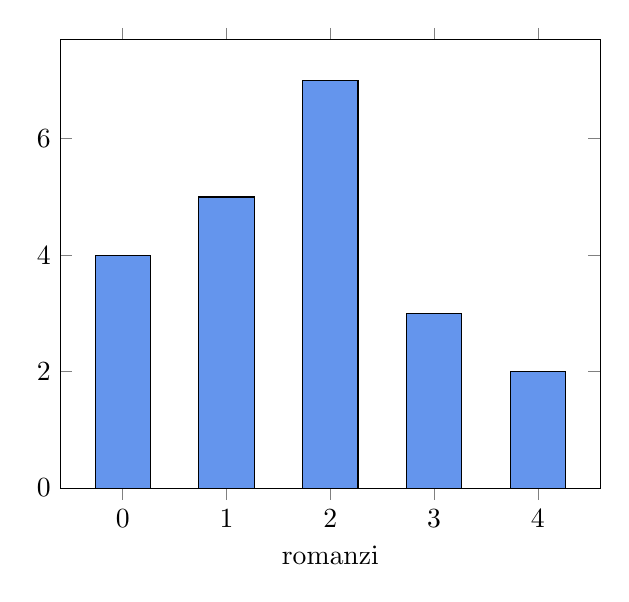
\begin{tikzpicture}
\begin{axis}[ymin=0,
ybar,
xlabel=romanzi,
bar width=20pt,enlarge x limits=0.15
]
    \addplot[fill=CornflowerBlue,draw=black]
      coordinates{
(0,4)
(1,5)
(2,7)
(3,3)
(4,2)
      };
\end{axis}
\end{tikzpicture}
\end{center}
\end{esercizio}
\pagebreak
\begin{esercizio}[Prove Invalsi~2004-2005]
\label{ese:A.58}
Il Ministero dell'Istruzione ha diffuso le seguenti informazioni sul numero di alunni stranieri della scuola italiana
nell'anno scolastico~2003-2004. La tabella riporta solo le~5 nazionalità più numerose.
\begin{center}
 \begin{tabularx}{.95\textwidth}{*{3}{X}}
\toprule
Nazionalità più numerose & Numero di alunni & Percentuale di alunni sul totale degli stranieri \\
\midrule
Albania & $\np{50000}$ & $\np{18,00}\%$ \\
Marocco & $\np{42000}$ & $\np{15,00}\%$ \\
Romania & $\np{28000}$ & $\np{10,00}\%$ \\
Cina    & $\np{16000}$ & $\np{6,00}\%$ \\
Ecuador & $\np{11000}$ & $\np{4,00}\%$ \\
\bottomrule
\end{tabularx}
\end{center}

Cosa si può dedurre da tali dati sugli alunni stranieri di nazionalità russa? Sono~$\ldots$
\begin{enumeratea}
 \item meno di~$\np{11000}$;
 \item sicuramente meno di~400;
 \item una percentuale compresa fra il~4\% e il~18\%;
 \item assenti dalle scuole italiane.
\end{enumeratea}
\end{esercizio}
\begin{esercizio}
\label{ese:A.59}
La tabella mostra la superficie delle varie province del Lazio.
\begin{center}
 \begin{tabular}{l*{5}{c}}
 \toprule
 Provincia & Frosinone & Latina & Rieti & Roma & Viterbo\\
 Superficie ($\unit{km}^2$) & $\np{3240}$& $\np{2251}$& $\np{2749}$& $\np{5352}$& $\np{3612}$\\
 \bottomrule
 \end{tabular}
\end{center}
Quale dei diagrammi riportati sotto descrive graficamente i dati della tabella?
\begin{center}
 % (c) 2012 Dimitrios Vrettos - d.vrettos@gmail.com


\begin{tikzpicture}[scale=.90,x=7mm,y=7mm]
  \draw (0,0) circle (3);
   \draw[fill=orange] (0,0) -- (0:3) arc (0:90:3);
 \draw[fill=brown] (0,0)-- (90:3) arc (90:133.2:3);
  \draw[fill=green] (0,0)-- (133.2:3) arc (133.2:198:3);
\draw[fill=red] (0,0)-- (198:3) arc (198:259.2:3);
\draw[fill=blue] (0,0)-- (259.2:3) arc (259.2:360:3);
\node[above] at (0,3) {1};

\begin{scope}[xshift=50mm]
  \draw (0,0) circle (3);
   \draw[fill=orange] (0,0) -- (0:3) arc (0:36:3);
 \draw[fill=brown] (0,0)-- (36:3) arc (36:64.8:3);
  \draw[fill=green] (0,0)-- (64.8:3) arc (64.8:180:3);
\draw[fill=red] (0,0)-- (180:3) arc (180:324.2:3);
\draw[fill=blue] (0,0)-- (324:3) arc (324:360:3);
\node[above] at (0,3) {2};
\end{scope}

\begin{scope}[xshift=100mm]
  \draw (0,0) circle (3);
   \draw[fill=orange] (0,0) -- (0:3) arc (0:39.6:3);
 \draw[fill=brown] (0,0)-- (39.6:3) arc (39.6:122.4:3);
  \draw[fill=green] (0,0)-- (122.4:3) arc (122.4:194.4:3);
\draw[fill=red] (0,0)-- (194.4:3) arc (194.4:309.6:3);
\draw[fill=blue] (0,0)-- (309.6:3) arc (309.6:360:3);
\node[above] at (0,3) {3};
\end{scope}


\begin{scope}[xshift=25mm, yshift=-50mm]
  \draw (0,0) circle (3);
   \draw[fill=orange] (0,0) -- (0:3) arc (0:68.4:3);
 \draw[fill=brown] (0,0)-- (68.4:3) arc (68.4:115.2:3);
  \draw[fill=green] (0,0)-- (115.2:3) arc (115.2:172.8:3);
\draw[fill=red] (0,0)-- (172.8:3) arc (172.8:284.4:3);
\draw[fill=blue] (0,0)-- (284.4:3) arc (284.4:360:3);
\node[above] at (0,3) {4};
\end{scope}

\begin{scope}[xshift=75mm, yshift=-50mm]
  \draw (0,0) circle (3);
   \draw[fill=orange] (0,0) -- (0:3) arc (0:126:3);
 \draw[fill=brown] (0,0)-- (126:3) arc (126:201.6:3);
  \draw[fill=green] (0,0)-- (201.6:3) arc (201.6:230.4:3);
\draw[fill=red] (0,0)-- (230.4:3) arc (230.4:304.4:3);
\draw[fill=blue] (0,0)-- (304.4:3) arc (304.4:360:3);
\node[above] at (0,3) {5};
\end{scope}

\begin{scope}[xshift=50mm, yshift=35mm]
\matrix[matrix of nodes, every node/.style={anchor=center}]{
\node[fill=orange]{};&Frosinone~~~~&
\node[fill=brown]{};&Latina~~~~&
\node[fill=green]{};&Rieti~~~~&
\node[fill=red]{};&Roma~~~~&
\node[fill=blue]{};&Viterbo\\};

\end{scope}
\end{tikzpicture}
\end{center}

\end{esercizio}

%\newpage
\subsection{Risposte}
\begin{multicols}{2}
 \paragraph{\thechapter.24.}
a)~$6$;\quad b)~$11$, $7$;\quad c)~$75$.

\paragraph{\thechapter.26.} $21$.

\paragraph{\thechapter.27.} $\np{7,1}$.

\paragraph{\thechapter.30.}
a)~$6$;\quad b)~$10$;\quad c)~$89$.

\paragraph{\thechapter.31.} $43$.

\paragraph{\thechapter.32.} $15$.

\paragraph{\thechapter.49.} $15$.

\paragraph{\thechapter.50.} d.
\end{multicols}

